%%%%%%%%%%%%   %%%%%%%%%%%%%%
\documentclass[12pt,onesided]{book}

\usepackage{amsmath}
\usepackage{latexsym}
\usepackage{amsfonts}
\usepackage[normalem]{ulem}
\usepackage{soul}
\usepackage{array}
\usepackage{amssymb}
\usepackage{extarrows}
\usepackage{graphicx}
%\usepackage[backend=biber,
%style=numeric,
%sorting=none,
%isbn=false,
%doi=false,
%url=false,
%]{biblatex}\addbibresource{bibliography.bib}

\usepackage{subfig}
\usepackage{wrapfig}
\usepackage{txfonts}
\usepackage{wasysym}
\usepackage{enumitem}
\usepackage{adjustbox}
\usepackage{ragged2e}
\usepackage[svgnames,table]{xcolor}
\usepackage{tikz}
\usepackage{longtable}
%\usepackage{changepage}
\usepackage{setspace}
\usepackage{hhline}
\usepackage{multicol}
\usepackage{tabto}
\usepackage{float}
\usepackage{multirow}
\usepackage{makecell}
\usepackage{fancyhdr}
\usepackage[toc,page]{appendix}
\usepackage[hidelinks]{hyperref}
\usetikzlibrary{shapes.symbols,shapes.geometric,shadows,arrows.meta}
\tikzset{>={Latex[width=1.5mm,length=2mm]}}
\usepackage{flowchart}
\usepackage[
paperheight=29.7 cm,
paperwidth=21 cm,
left=1.25in,
right=1.25in,
top=1.0in,
bottom=1.0in,
headheight=1in]{geometry}
\usepackage[utf8]{inputenc}
\usepackage[T1]{fontenc}
\TabPositions{0.5in,1.0in,1.5in,2.0in,2.5in,3.0in,3.5in,4.0in,4.5in,5.0in,5.5in,}
\usepackage{mathptmx}% Times Roman font
\urlstyle{same}

\usepackage[croatian]{babel}
\usepackage{setspace}
\usepackage{lipsum}
\makeatletter
\setlength{\@fptop}{0 pt}
\makeatother
\graphicspath{{Slike/}}

\renewcommand{\thefootnote}{\fnsymbol{footnote}}


 %%%%%%%%%%%% Literatura  %%%%%%%%%%%%%%
\usepackage[square,numbers,sort]{natbib}

%\pgfplotsset{
%	legend entry/.initial=,
%	every axis plot post/.code={%
%		\pgfkeysgetvalue{/pgfplots/legend entry}\tempValue
%		\ifx\tempValue\empty
%		\pgfkeysalso{/pgfplots/forget plot}%
%		\else
%		\expandafter\addlegendentry\expandafter{\tempValue}%
%		\fi
%	},
%}


 %%%%%%%%%%%%  Set Depths for Sections  %%%%%%%%%%%%%%

% 1) Section
% 1.1) SubSection
% 1.1.1) SubSubSection
% 1.1.1.1) Paragraph
% 1.1.1.1.1) Subparagraph


\setcounter{tocdepth}{5}
\setcounter{secnumdepth}{5}


 %%%%%%%%%%%%  Set Depths for Nested Lists created by \begin{enumerate}  %%%%%%%%%%%%%%


\setlistdepth{9}
\renewlist{enumerate}{enumerate}{9}
		\setlist[enumerate,1]{label=\arabic*)}
		\setlist[enumerate,2]{label=\alph*)}
		\setlist[enumerate,3]{label=(\roman*)}
		\setlist[enumerate,4]{label=(\arabic*)}
		\setlist[enumerate,5]{label=(\Alph*)}
		\setlist[enumerate,6]{label=(\Roman*)}
		\setlist[enumerate,7]{label=\arabic*}
		\setlist[enumerate,8]{label=\alph*}
		\setlist[enumerate,9]{label=\roman*}

\renewlist{itemize}{itemize}{9}
		\setlist[itemize]{label=$\cdot$}
		\setlist[itemize,1]{label={--}}
		\setlist[itemize,2]{label=$\circ$}
		\setlist[itemize,3]{label=$\ast$}
		\setlist[itemize,4]{label=$\dagger$}
		\setlist[itemize,5]{label=$\triangleright$}
		\setlist[itemize,6]{label=$\bigstar$}
		\setlist[itemize,7]{label=$\blacklozenge$}
		\setlist[itemize,8]{label=$\prime$}



 %%%%%%%%%%%%  Header here  %%%%%%%%%%%%%%


%\pagestyle{fancy}
%\fancyhf{}
%%\cfoot{ 
%%\vspace{\baselineskip}
%%}
%\fancyfoot[R]{\thepage}
%%\fancyfoot[L]{\thepage}
%\renewcommand{\headrulewidth}{0pt}
%\setlength{\topsep}{0pt}\setlength{\parindent}{0pt}
%\renewcommand{\arraystretch}{1.3}

\pagestyle{fancy} % Turn on the style
\fancyhf{} % Start with clearing everything in the header and footer
% Set the right side of the footer to be the page number
\fancyfoot[LE,RO]{\thepage}

% Redefine plain style, which is used for titlepage and chapter beginnings
% From https://tex.stackexchange.com/a/30230/828
\fancypagestyle{plain}{%
	\renewcommand{\headrulewidth}{0pt}%
	\fancyhf{}%
	\fancyfoot[R]{\thepage}%
}


%%%%%%%%%%%%%%%%%	Naslovi bez aoisd	%%%%%%%%%%%%%%%%%%%%%%%%%%%

\makeatletter
\def\@makechapterhead#1{%
	\vspace*{50\p@}%
	{\parindent \z@ \raggedright \normalfont
		\ifnum \c@secnumdepth >\m@ne
		\if@mainmatter
		\Huge\bfseries \thechapter.\space%
		%\par\nobreak
		%\vskip 20\p@
		\fi
		%
		\Huge \bfseries \uppercase{#1}\par\nobreak
		\vskip 40\p@
		
	
}}
\makeatother





\usepackage{titlesec}



%%%%%%%%%%%%%%%%%%%% Document code starts here %%%%%%%%%%%%%%%%%%%%

\newcommand{\autor} {Fredrik Lamb}
\newcommand{\studij} {Preddiplomski sveučilišni}
\newcommand{\smjer} {Pozitivan}
\newcommand{\kolegij} {Filozofija građevinarstva}
\newcommand{\naslov}{Tko pije, a tko plaća na neaktivnom gradilištu?}
\newcommand{\JMBAG} {000111222}
\newcommand{\vrsta}{Završni rad} % ili Diplomski





%%



\onehalfspacing

%%%%%%%%%%%%%%%%%%%% Document code starts here %%%%%%%%%%%%%%%%%%%%
%%%%%%%%%%%%%%%%%%%% Enter the data %%%%%%%%%%%%%%%%%%%%

\newcommand{\autor} {Fredrik Lamb}
\newcommand{\studij} {Preddiplomski sveučilišni}
\newcommand{\smjer} {Pozitivan}
\newcommand{\kolegij} {Filozofija građevinarstva}
\newcommand{\naslov}{Tko pije, a tko plaća na neaktivnom gradilištu?}
\newcommand{\JMBAG} {000111222}
\newcommand{\vrsta}{Završni rad} % ili Diplomski

%%%%%%%%%%%%%%%%%%%%%%%%%%%%%%%%%%%%%%%%
\begin{document}

\thispagestyle{empty}

\vspace{\baselineskip}
\begin{Center}
{\fontsize{14pt}{16.8pt}\selectfont 
\textbf{SVEUČILIŠTE U RIJECI}\par}
\end{Center}\par

\begin{Center}
{\fontsize{14pt}{16.8pt}\selectfont \textbf{GRAĐEVINSKI FAKULTET}\par}
\end{Center}\par


\vspace{\baselineskip}
\begin{Center}
{\fontsize{14pt}{16.8pt}\selectfont \par \textbf{{\studij}}\par}
\end{Center}\par

\begin{Center}
{\fontsize{14pt}{16.8pt}\selectfont \textbf{{\smjer}}\par}
\end{Center}\par

\begin{Center}
{\fontsize{14pt}{16.8pt}\selectfont \textbf{ {\kolegij} }\par}
\end{Center}\par


%\vspace{\baselineskip}
%
%\vspace{\baselineskip}
%
%\vspace{\baselineskip}
%
%\vspace{\baselineskip}
%
%%\vspace{\baselineskip}
%
%%\vspace{\baselineskip}
%
%\vspace{\baselineskip}
%
%\vspace{\baselineskip}
%
%\vspace{\baselineskip}
%
%\vspace{\baselineskip}
%
%\vspace{\baselineskip}
%
%\vspace{\baselineskip}

\vskip 144pt

\begin{Center}
{\fontsize{14pt}{16.8pt}\selectfont \textbf{{\autor}}\par}
\end{Center}\par

\begin{Center}
{\fontsize{14pt}{16.8pt}\selectfont \textbf{\JMBAG}\par}
\end{Center}\par


\vspace{\baselineskip}

\vspace{\baselineskip}

\vspace{\baselineskip}
\begin{Center}
{\fontsize{14pt}{16.8pt}\selectfont \textbf{ {\naslov} }\par}
\end{Center}\par


\vspace{\baselineskip}

\vspace{\baselineskip}

\vspace{\baselineskip}
\begin{Center}
\textbf{{\vrsta}}
\end{Center}\par


\vspace{\baselineskip}

\vspace{\baselineskip}

\vspace{\baselineskip}

\vspace{\baselineskip}

\vspace{\baselineskip}

\vspace{\baselineskip}

\vspace{\baselineskip}

\vspace{\baselineskip}

\vspace{\baselineskip}
\begin{Center}
\textbf{Rijeka, {\today}}
\end{Center}\par

%\begin{justify}


 %%%%%%%%%%%%  Starting New Page here %%%%%%%%%%%%%%

\newpage

\thispagestyle{empty}
\mbox{}
\thispagestyle{empty}

\newpage


\thispagestyle{empty}
\mbox{}
\thispagestyle{empty}


\vskip 48 pt

\begin{center}
{\fontsize{14pt}{16.8pt}\selectfont \textbf{IZJAVA}\par}\par
\end{center}\par

\vspace{\baselineskip}

\vspace{\baselineskip}

\begin{justify}
	\begin{onehalfspace}
\vrsta izradio/izradila sam samostalno, u suradnji s mentorom/mentoricom i uz poštivanje pozitivnih građevinskih propisa i znanstvenih dostignuća iz područja građevinarstva. Građevinski fakultet u Rijeci je nositelj prava intelektualnog vlasništva u odnosu na ovaj rad.
This is a test.
	\end{onehalfspace}

\end{justify}\par

\vspace{\baselineskip}

\vspace{\baselineskip}

\vspace{\baselineskip}
\_\_\_\_\_\_\_\_\_\_\_\_\_\_\_\_\_\_\_\_\_\_\_\_\_\_\_\_\_\_\_\_\_\_\_\_\_\_\_\_\_\_ \par

{\autor}\par



\vskip 60 pt
U Rijeci, {\today}\par

\newpage

\thispagestyle{empty}
\mbox{}
\thispagestyle{empty}

\pagestyle{empty}
\input{./Poglavlja/zahvale}

\cleardoublepage

\pagenumbering{roman}
\setcounter{page}{1}

\chapter*{\uppercase{Sa\v{z}etak}}

\cleardoublepage
\setcounter{page}{1}

\tableofcontents
\cleardoublepage

\listoffigures
\addcontentsline{toc}{chapter}{\listfigurename}

\cleardoublepage
\listoftables
\addcontentsline{toc}{chapter}{\listtablename}

\clearpage

\pagenumbering{arabic}
\pagestyle{plain}
\setcounter{page}{1}

\chapter{\uppercase{rand}}
\label{ch:rand}
\pagenumbering{arabic}
\setcounter{page}{1}

\lipsum

\cite{Peiris1970,Massoudi2001}


\begin{itemize}
	\item paps
	\item asdasda
\end{itemize}
\cleardoublepage
\chapter{\uppercase{Poglavlje 2}}


\lipsum[1-3]


\begin{table}
	\centering
	\caption{Nesto malo duži tekst}
	\label{tab:red}
	\begin{tabular}{c c c c}
		\hline
		rbr & Pomak & sigma 1 & u \\ \hline
		1 & 0 0.14 0.35 0.7 1.4 2.8 7 14 & 450 & 0 \\ \hline
		2 & 1.542 & 540 & 45 \\ \hline
		3 & 1.752 & 650 & 105 \\ \hline
		4 & 2.102 & 790 & 190 \\ \hline
		5 & 2.802 & 850 & 235 \\ \hline
		6 & 4.202 & 840 & 245 \\ \hline
		7 & 8.402 & 810 & 260 \\ \hline
		8 & 15.402 & 790 & 270 \\ \hline
	\end{tabular}
\end{table}


\lipsum[1-3] \cite{Massoudi2001}
\cleardoublepage
\chapter{\uppercase{title}}
\lipsum[1-3]


\section{title}

\lipsum[1-3]


\begin{figure}
	\centering
	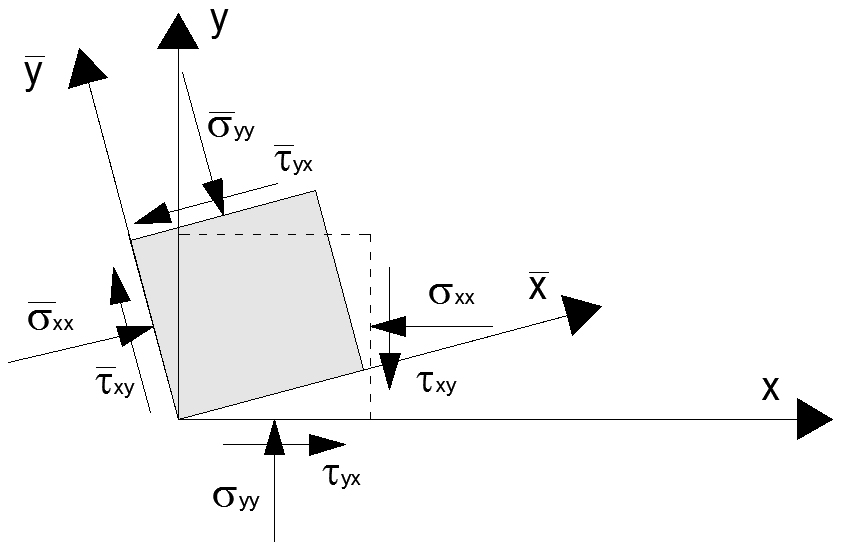
\includegraphics[width=0.7\linewidth]{Slike/2dtrans}
	\caption{sdadadasda}
	\label{fig:2dtrans}
\end{figure}


\subsection{\textit{title}}


\lipsum[1-3]

\begin{figure}
	\centering
	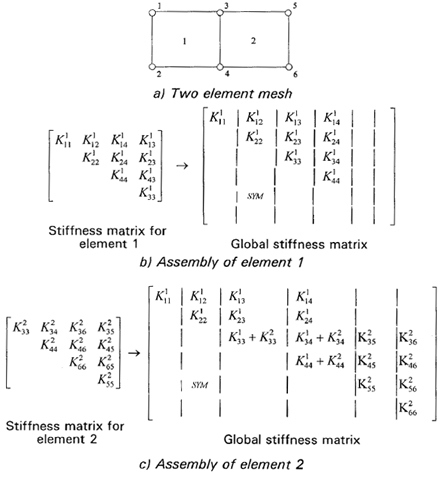
\includegraphics[width=0.7\linewidth]{Slike/assembly}
	\caption{Nedostaje caption}
	\label{fig:assembly}
\end{figure}


\lipsum[1-3] \cite{Gutierrez2009,doi:10.1680/geot.1986.36.1.65,krahn}
\lipsum[1-3]

\begin{figure}
	\begin{tikzpicture}% table
\begin{axis}[
xlabel=$D_{p,min}$,
ylabel=$\eta_{max}$,
width = 0.9 \textwidth,
height = 0.7 \textwidth,
legend pos = south east,
grid =  both,
xmin = -0.8,
xmax = 0.2,
ymin = 0.8,
ymax = 1.6,
x dir = reverse,
legend style = {font = \footnotesize},
]
\addplot [domain = -1:0.2, thick, dashed, line width = 1.5 pt,color = black, legend entry = ${M = 1.345}$] {1.345 - 0.3*x};
\addplot [only marks, color = black] table[x=dminC,y=etamaxC, col sep = tab] {./dataset/etadil.txt};
\addplot [thin, color = black, dashed,mark = none, legend entry = \citep{cornforth1961plane} ] coordinates {
(0,1.2602)
(-0.8,1.763)
};
%
\addlegendimage{empty legend};
\addlegendentry{\citep{jeffShut}};
\addlegendimage{empty legend};
\addlegendentry{\citep{vaid1992strength}};
\addplot [thin, color = black,dashed, mark = none,% legend entry = ${[60],[61]}$
] coordinates {
	(0,1.267)
	(-0.7502,1.8)
};

\addplot [domain = 0:0.2,dotted] {-0.708777*x+1.267};
\addplot [domain = 0:0.2,dotted] {-0.6285*x+1.2602};
%
\addplot+[name path = A, mark = none]coordinates {
(0.2,1.22)
(-0.8,1.52)
};		%old
\addplot+[name path = B, mark = none]{-0.3*x+1.41};		%old unfit
\addplot[gray!50,opacity = 0.3, legend entry = Data Range] fill between[of=A and B];

\draw [decorate,decoration={brace,amplitude=10pt,mirror,raise=4pt}]
(axis cs:0.2,1.125) -- (axis cs:0,1.2602) node [black,midway,xshift=50 pt, yshift = -12 pt] {\footnotesize
	Assumed extensions };
\node [font = \footnotesize] at (axis cs: -0.07,1.10) {according to: };
\node [font = \footnotesize, fill = white] at (axis cs:-0.05,1.05) {  \citep{cornforth1961plane}};
\node [font = \footnotesize, fill = white] at (axis cs:-0.05,1.00) {  \citep{jeffShut}};
\node [font = \footnotesize, fill = white] at (axis cs:-0.05,0.950) {  \citep{vaid1992strength}};

\end{axis}

\end{tikzpicture}
\end{figure}

\cleardoublepage\phantomsection

%\printbibliography
\vspace{\baselineskip}
%\label{Bibliography}
\renewcommand{\bibname}{\uppercase{Literatura}}
\addcontentsline{toc}{chapter}{\textbf{Literatura}}
\bibliographystyle{unsrtnat-GFRI}
\bibliography{bibliography}
%\bibliographystyle{vancouver}
\end{document}